%==========================================================================
%  TRES0312 Fysikk — Foiler-mal
%
%  MØrk/lys modus: kommenter ut én av de to linjene nedenfor.
%==========================================================================
\newif\ifdarkmode
\darkmodetrue      % ← mørk modus
%\darkmodefalse   % ← lys modus  (fjern % foran og legg % foran linjen over)

\documentclass[aspectratio=169, 12pt]{beamer}

\usepackage{amd-beamer}
\usetikzlibrary{overlay-beamer-styles}
\usetikzlibrary{calc}

%--------------------------------------------------------------------------
%  DOKUMENTINFO
%--------------------------------------------------------------------------
\title{Fluider, massetetthet og trykk}
\subtitle{TRES0312 --- kapittel 7.1}
\author{Ben David Normann}
\date{\today}

%--------------------------------------------------------------------------
%  SEKSJONSKONTEKST
%--------------------------------------------------------------------------
\setcounter{section}{7}   % Kapittel 7: "Fluiddynamikk"

\begin{document}

%--------------------------------------------------------------------------
%  SLIDE 1 — TITTELSIDE
%--------------------------------------------------------------------------
\begin{frame}[plain]
  \titlepage
  \dekkerdelkap{kapittel 7.1}
  \vspace{0.3cm}
  \begin{center}
  {\bfseries\color{repcol} Første time: massetetthet og trykk. Etter pausen: lufttrykk.}
  \end{center}
\end{frame}

%--------------------------------------------------------------------------
%  SLIDE 2 — Tre kjappe fra forrige gang
%--------------------------------------------------------------------------
\begin{frame}{}

  \repetisjon{Tre kjappe fra forrige gang}{%
    \begin{enumerate}[1.]
      \item Hvilke to betingelser må være oppfylt for fullstendig statisk likevekt?
      \item Hvordan regner vi ut massesenteret $x_\text{ms}$ til flere masser langs en akse?
      \item Hvorfor lønner det seg å velge punktet der flest ukjente krefter angriper, når vi regner kraftmoment?
    \end{enumerate}
  }

\end{frame}

%==========================================================================
%  DEL 1: FLUIDER, MASSETETTHET OG TRYKK (7.1.1--7.1.2)
%==========================================================================

%--------------------------------------------------------------------------
%  SLIDE 3 — Hva er et fluid?
%--------------------------------------------------------------------------
\begin{frame}{Hva er et fluid?}

  Et \textbf{fluid} er et stoff som kan \textit{flyte} og ta formen til beholderen det er i.
  \begin{itemize}
    \item \textbf{Væsker} (vann, olje): har et bestemt volum, men ingen fast form.
    \item \textbf{Gasser} (luft): har verken fast form eller fast volum. De fyller hele beholderen.
  \end{itemize}

\end{frame}

%--------------------------------------------------------------------------
%  SLIDE 4 — Til ettertanke: stålskip
%--------------------------------------------------------------------------
\begin{frame}{Massetetthet}

  \tanke{}{%
  Skip med skrog av metall flyter, enda metall er tyngre enn vann. Hvordan kan det ha seg?
  }
  \pause
  \svar{
  Det er ikke massen alene som avgjør, men hvor mye masse som er pakket inn i et gitt volum. Skipet som helhet (stål \textit{pluss} all lufta inni) har mindre masse per volum enn vann. Vi trenger altså begrepet \textit{massetetthet}.
  }

\end{frame}

%--------------------------------------------------------------------------
%  SLIDE 5 — Definisjon: massetetthet
%--------------------------------------------------------------------------
\begin{frame}{Massetetthet}

  \begin{columns}[T]
    \begin{column}{0.55\textwidth}
      \defnat{7.1.1}{Massetetthet}{
      Massetettheten $\rho$ (rho) til et stoff er
      \[
        \rho = \frac{m}{V}
      \]
      der $m$ er massen og $V$ er volumet. Enheten er $\mathrm{kg/m^3}$ (eller $\mathrm{g/cm^3}$).
      }
    \end{column}
    \begin{column}{0.42\textwidth}
      \centering
      \small
      \begin{tabular}{lr}
        \textbf{Stoff} & $\rho$ ($10^3\,\mathrm{kg/m^3}$) \\
        \hline
        Gull & 19.3 \\
        Stål & 7.85 \\
        Aluminium & 2.70 \\
        Sjøvann & 1.03 \\
        Vann & 1.0 \\
        Is & 0.92 \\
        Luft & 0.0012 \\
      \end{tabular}
    \end{column}
  \end{columns}

  \pause
  \merk{Lurt å huske:}{%
  1 liter vann har en masse på omtrent 1 kg.
  }

\end{frame}

%--------------------------------------------------------------------------
%  SLIDE 6 — Aktivitet: vann og metall
%--------------------------------------------------------------------------
%  Fasit: a) V = 2.5e-3 m^3, m = 1.0e3 * 2.5e-3 = 2.5 kg.
%         b) V = (2.0 cm)^3 = 8.0 cm^3, rho = 22 g / 8.0 cm^3 = 2.75 g/cm^3 ≈ 2.8e3 kg/m^3
%            -> nærmest aluminium (2.70).
\begin{frame}{Aktivitet}

  \aktivitet{Vann og metall}{%
  \begin{enumerate}[a)]
    \item Hva er massen til $2.5\,\mathrm{L}$ vann? \textit{(Hint: $1\,\mathrm{L} = 1\,\mathrm{dm^3} = 10^{-3}\,\mathrm{m^3}$.)}
    \item En liten metallterning har sidekanter på $2.0\,\mathrm{cm}$ og masse $22\,\mathrm{g}$. Finn massetettheten. Hvilket metall er terningen trolig laget av?
  \end{enumerate}
  }

\end{frame}

%--------------------------------------------------------------------------
%  SLIDE 7 — Til ettertanke: legokloss
%--------------------------------------------------------------------------
\begin{frame}{Trykk}

  \tanke{}{%
  Hvorfor gjør det så vondt å tråkke på en legokloss, mens det ikke gjør vondt å stå på gulvet med hele foten?
  }
  \pause
  \svar{
  Kraften fra kroppen er like stor i begge tilfeller. Men på legoklossen fordeles kraften over et mye mindre areal. Det som avgjør hvor vondt det gjør, er kraften \textit{per areal}: \textit{trykket}.
  }

\end{frame}

%--------------------------------------------------------------------------
%  SLIDE 8 — Definisjon: trykk
%--------------------------------------------------------------------------
\begin{frame}{Trykk}

  \defnat{7.1.2}{Trykk}{
  Trykket $p$ er kraften $F$ som virker \textit{vinkelrett} på en flate, delt på arealet $A$ til flaten:
  \[
    p = \frac{F}{A}
  \]
  Enheten er pascal: $1\,\mathrm{Pa} = 1\,\mathrm{N/m^2}$.
  }

  \pause
  \merk{Trykk er ikke en vektor!}{%
  Trykk har bare en størrelse, ingen retning. Det er \textit{kraften} fra trykket som har retning: den står alltid vinkelrett på flaten.
  }

\end{frame}

%--------------------------------------------------------------------------
%  SLIDE 9 — Aktivitet: ski eller støvler
%--------------------------------------------------------------------------
%  Fasit: F = m g = 80*9.81 = 784.8 N.
%         a) p = 784.8 / 0.060 = 1.31e4 Pa ≈ 13 kPa.
%         b) A = 2*1.9*0.065 = 0.247 m^2, p = 784.8/0.247 = 3.18e3 Pa ≈ 3.2 kPa.
%         c) Samme kraft, ca. 4 ganger så stort areal -> ca. 4 ganger mindre trykk.
\begin{frame}{Aktivitet}

  \begin{columns}[T]
    \begin{column}{0.60\textwidth}
      \aktivitet{Ski eller støvler?}{%
      En person med masse $m = 80\,\mathrm{kg}$ står på snø.
      \begin{enumerate}[a)]
        \item Finn trykket mot snøen når personen står i støvler. De to sålene har til sammen areal $0.060\,\mathrm{m^2}$.
        \item Hver ski er $1.9\,\mathrm{m}$ lang og $6.5\,\mathrm{cm}$ bred. Finn trykket mot snøen med ski.
        \item Hvorfor synker man mindre ned med ski?
      \end{enumerate}
      }
    \end{column}
    \begin{column}{0.38\textwidth}
      \centering
      \vspace{10mm}
      \begin{tikzpicture}[scale=0.9]
        % Snø
        \fill[white!70!oppgcol] (-0.2,-0.25) rectangle (4.2,0);
        % Støvel
        \fill[gray!70] (0.2,0) rectangle (0.9,0.25);
        \fill[gray!70] (0.2,0.25) rectangle (0.55,1.0);
        \node[font=\footnotesize] at (0.55,1.3) {støvel};
        % Ski
        \fill[headCol!60!white] (1.4,0) rectangle (4.0,0.08);
        \fill[gray!70] (2.4,0.08) rectangle (3.0,0.33);
        \fill[gray!70] (2.4,0.33) rectangle (2.7,1.0);
        \node[font=\footnotesize] at (2.7,1.3) {ski};
      \end{tikzpicture}
    \end{column}
  \end{columns}

\end{frame}

%--------------------------------------------------------------------------
%  SLIDE 10 — Trykk på mikroskopisk nivå
%--------------------------------------------------------------------------
\begin{frame}{Trykk på mikroskopisk nivå}

  \begin{columns}[c]
    \begin{column}{0.55\textwidth}
      \begin{itemize}
        \item En gass består av molekyler som farer rundt i alle retninger.
        \item Hver gang et molekyl treffer veggen, dytter det litt på den.
        \item Summen av alle disse små dyttene, per areal, er \textit{trykket}.
      \end{itemize}
    \end{column}
    \begin{column}{0.42\textwidth}
      \centering
      \begin{tikzpicture}[scale=1.0, >={Stealth[length=5pt,width=4pt]}]
        \draw[very thick, textcolor] (0,0) rectangle (4,3);
        \foreach \x/\y/\a in {0.6/0.7/30, 1.5/2.2/-40, 2.4/1.1/150, 3.3/2.4/210, 1.0/1.6/80,
                              2.9/0.5/20, 3.4/1.5/-20, 2.0/2.6/250, 0.5/2.5/-70, 1.8/0.4/100}{
          \fill[oppgcol!70!white] (\x,\y) circle (0.09);
          \draw[->, thin, textcolor!80] (\x,\y) -- ++(\a:0.45);
        }
      \end{tikzpicture}
    \end{column}
  \end{columns}

\end{frame}

\begin{frame}{Trykk på mikroskopisk nivå}

  \tanke{}{%
  Hva skjer med trykket hvis molekylene beveger seg raskere?
  }
  \pause
  \svar{
  De treffer veggen oftere og hardere, så trykket øker.
  }

\end{frame}

%--------------------------------------------------------------------------
%  SLIDE 11 — Oppsummering: massetetthet og trykk
%--------------------------------------------------------------------------
\begin{frame}{}

  \oppsum{Massetetthet og trykk}{%
  \begin{enumerate}[1.]
    \item[] Massetetthet: $\rho = m/V$. 1 L vann har masse ca. 1 kg.
    \item[] Trykk: $p = F/A$, der $F$ står vinkelrett på flaten. Enhet: $\mathrm{Pa} = \mathrm{N/m^2}$.
    \item[] Samme kraft over et mindre areal gir større trykk.
    \item[] Trykk er en skalar. Kraften fra trykket står vinkelrett på flaten.
  \end{enumerate}
  }

\end{frame}

%--------------------------------------------------------------------------
%  SLIDE 12 — PAUSE
%--------------------------------------------------------------------------
\begin{frame}
\begin{center}
  \Huge{Pause}\\[8pt]
  {\large Etter pausen: lufttrykk}
\end{center}
\end{frame}

%==========================================================================
%  DEL 2: LUFTTRYKK (7.1.3)
%==========================================================================

%--------------------------------------------------------------------------
%  SLIDE 13 — Til ettertanke: sugekopper
%--------------------------------------------------------------------------
\begin{frame}{Lufttrykk}

  \tanke{}{%
  Hvorfor fungerer sugekopper?
  }
  \pause
  \svar{
  Når du presser sugekoppen mot en flate, presses lufta ut under den. Lufta utenfor presser koppen inn mot flaten. Det er altså \textit{lufttrykket} som holder sugekoppen fast. Jo større sugekopp, desto større kraft.
  }

\end{frame}

%--------------------------------------------------------------------------
%  SLIDE 14 — Lufttrykk og 1 atm
%--------------------------------------------------------------------------
\begin{frame}{Lufttrykk}

  \begin{itemize}
    \item Vi lever på bunnen av et «hav» av luft.
    \item Lufta har vekt, og presser på alt den omgir, fra \textit{alle kanter}.
    \item Lufttrykket ved havoverflaten kalles \textit{én atmosfære} (1 atm):
  \end{itemize}

  \graabox{$\displaystyle 1\,\mathrm{atm} = 101\,325\,\mathrm{Pa} \approx 1.013\cdot 10^5\,\mathrm{Pa}$}

\end{frame}

\begin{frame}{Lufttrykk}

  \tanke{}{%
  Hvis du pumper ut all lufta fra et rom, hva skjer med sugekoppene på veggene?
  }
  \pause
  \svar{
  De faller av. Uten luft i rommet er det ingenting som presser dem mot veggen.
  }

\end{frame}

%--------------------------------------------------------------------------
%  SLIDE 15 — Aktivitet: lufta presser på et bord
%--------------------------------------------------------------------------
%  Fasit: A = 1.5*0.90 = 1.35 m^2.
%         a) F = 1.013e5*1.35 = 1.37e5 N ≈ 1.4e5 N.
%         b) m = F/g = 1.39e4 kg ≈ 1.4e4 kg (omtrent 14 tonn).
\begin{frame}{Aktivitet}

  \aktivitet{Lufta presser på et bord}{%
  Et bord har en rektangulær bordplate som er $1.5\,\mathrm{m}$ lang og $0.90\,\mathrm{m}$ bred. Lufttrykket er $p_0 = 1.013\cdot 10^5\,\mathrm{Pa}$.
  \begin{enumerate}[a)]
    \item Finn kraften fra lufta på oversiden av bordplata.
    \item Hvor stor masse ville hatt en like stor tyngde?
  \end{enumerate}
  }

\end{frame}

\begin{frame}{Lufttrykk}

  \tanke{}{%
  Lufta presser på bordplata med en kraft som tilsvarer tyngden av omtrent 14 tonn. Hvorfor knekker ikke bordet sammen?
  }
  \pause
  \svar{
  Lufta presser like mye på \textit{undersiden} av bordplata. Kreftene oppover og nedover opphever hverandre.
  }

  \pause
  \vspace{-3mm}
  \begin{center}
  \begin{minipage}{0.24\textwidth}
    \href{https://www.nrk.no/video/132654}{%
    \begin{tikzpicture}[inner sep=0pt]
      \node (thumb) {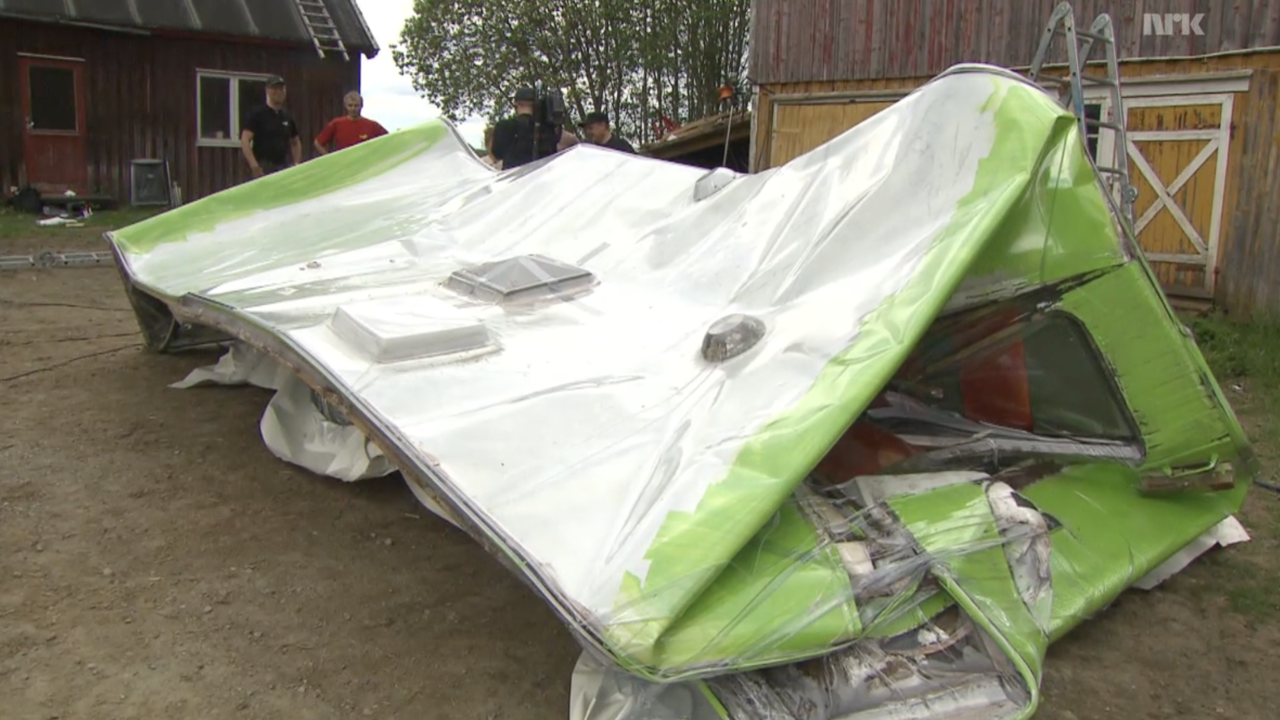
\includegraphics[width=\linewidth]{Images/NRK_Campingvogn.png}};
      \fill[black, opacity=0.55] (thumb.center) circle (0.42cm);
      \draw[white, line width=1.2pt] (thumb.center) circle (0.42cm);
      \fill[white] ($(thumb.center)+(-0.13,-0.2)$) -- ($(thumb.center)+(-0.13,0.2)$) -- ($(thumb.center)+(0.22,0)$) -- cycle;
    \end{tikzpicture}}%
  \end{minipage}%
  \hspace{5mm}%
  \begin{minipage}{0.45\textwidth}
    \small Men hva skjer hvis lufta bare presser fra \textit{én} side? Se hva som skjer med en campingvogn når lufta inni den pumpes ut. \textit{(Videoklipp fra NRK --- klikk på bildet.)}
  \end{minipage}
  \end{center}

\end{frame}

%--------------------------------------------------------------------------
%  SLIDE 16 — Overtrykk
%--------------------------------------------------------------------------
\begin{frame}{Overtrykk}

  \begin{itemize}
    \item Inne i et bildekk er trykket \textit{større} enn lufttrykket utenfor.
    \item En dekktrykkmåler viser \textbf{overtrykket} $\Delta p$: hvor mye større trykket er enn lufttrykket rundt.
  \end{itemize}

  \graabox{$\displaystyle p = p_0 + \Delta p$}

  \pause
  \merk{Enheten bar}{%
  Dekktrykk oppgis ofte i bar: $1\,\mathrm{bar} = 1.0\cdot 10^5\,\mathrm{Pa}$, altså omtrent 1 atm.
  }

\end{frame}

%--------------------------------------------------------------------------
%  SLIDE 17 — Aktivitet: lufttrykk i bildekk
%--------------------------------------------------------------------------
%  Fasit: a) p = 1.013e5 + 2.5e5 = 3.51e5 Pa ≈ 3.5e5 Pa; 3.51e5/1.013e5 = 3.47 ≈ 3.5 atm.
%         b) F = 1500*9.81/4 = 3679 N; A = F/Δp = 3679/2.5e5 = 1.47e-2 m^2 ≈ 1.5e-2 m^2 (ca. 150 cm^2).
\begin{frame}{Aktivitet}

  \aktivitet{Lufttrykk i bildekk}{%
  En trykkmåler viser at overtrykket i et bildekk er $2.5\,\mathrm{bar}$. Lufttrykket utenfor er $p_0 = 1.013\cdot 10^5\,\mathrm{Pa}$.
  \begin{enumerate}[a)]
    \item Finn det totale trykket inne i dekket. Hvor mange atmosfærer er det?
    \item Bilen har masse $1500\,\mathrm{kg}$, fordelt likt på fire hjul. Det er overtrykket som bærer bilen. Hvor stort areal av hvert dekk ligger an mot veien?
  \end{enumerate}
  }

\end{frame}

\begin{frame}{Overtrykk}

  \tanke{}{%
  Hva skjer med flaten som ligger an mot veien hvis dekktrykket er for lavt? Hvorfor bruker bilen da mer drivstoff?
  }
  \pause
  \svar{
  Med lavere overtrykk må en større del av dekket ligge an mot veien for å bære bilen ($A = F/\Delta p$). Dekket blir flatere og deformeres mer når det ruller, og det koster energi.
  }

\end{frame}

%--------------------------------------------------------------------------
%  SLIDE 18 — Oppsummering: lufttrykk
%--------------------------------------------------------------------------
\begin{frame}{}

  \oppsum{Lufttrykk}{%
  \begin{enumerate}[1.]
    \item[] Lufta har vekt og presser på alt fra alle kanter.
    \item[] $1\,\mathrm{atm} = 101\,325\,\mathrm{Pa} \approx 1.013\cdot 10^5\,\mathrm{Pa}$.
    \item[] Kraften fra lufttrykket kan bli stor, men den virker som regel fra begge sider.
    \item[] Overtrykk: $p = p_0 + \Delta p$. Dekktrykkmålere viser $\Delta p$.
  \end{enumerate}
  }

\end{frame}

%--------------------------------------------------------------------------
%  SLIDE 19 — Neste gang
%--------------------------------------------------------------------------
\begin{frame}
\begin{center}
  \Huge{Neste gang: trykk i væsker}
  \vspace{6mm}
\end{center}
\end{frame}

\end{document}
